\chapter{The Spectrum of the Hydrogen Atom}
\section{Introduction}
In this experiment we will observe the discrete light spectrum one observes due to the atomic electron transition in a gas discharge lamp. We will see that the spectrum consists of a collection of sharp, single colored lines corresponding to the discrete atomic energy levels of the gas atoms. Wit our experimental setup, we will be able to measure the wavelength of the light emitted quite precisely; usually better than one part in one thousand. It is therefore crucial to make all calculations to five  significant figures.

\section{Theory}
\subsection{The Spectrum of the Hydrogen Atom}
According to the classical theory of electromagnetism, atoms should radiate continuously which would cause the electrons to lose energy and fall into the nuclei within a short timespan. Obviously this is not the case since we have stable atoms. Something must be wrong with this classical description.\myskip

Niels Bohr postulated an alternative theory for atoms, suggesting that the electrons can only exist in certain discrete energy states and they may only jump between these states discontinuously. This discontinuity explains why we see a collection of sharp lines in a gas discharge lamp, and not a continuous spectrum as in a usual light bulb. \myskip

Bohr was able to derive the following formula for the energy of the energy levels only using natural constants
\begin{equation}
  E_{n}=-\frac{2\pi^2 me^4k^{2}_{e}}{n^2h^2}=-\frac{me^4}{h^2}\bigg(\frac{1}{8\varepsilon^{2}_{0}}\bigg)\frac{1}{n^2}
\end{equation}
Therefore the energy one gets for a transition from an initial level $n_i$ to a final level $n_f$ is $\Delta E = E_{n_{i}} - E_{n_{f}}$.\myskip

This transition energy is released in the form of light and one can relate it to the photon wavelength via
\begin{equation}
  \frac{1}{\lambda}=\frac{f}{c}=\frac{\Delta E}{hc}=\frac{E_{n_{i}}-E_{n_{f}}}{hc}=R\bigg(\frac{1}{n^2_{f}}-\frac{1}{n^2_{i}}\bigg)
\label{eq:lambda}
\end{equation}
where $R$ is called the Rydberg constant, which is given by
\begin{equation}
  R=\frac{2\pi^2me^4k^2_{e}}{h^3c}=1.0974\times 10^{7}\, \mathrm{m}^{-1}
\end{equation}

\subsection{Resolving a Light Spectrum with a Grating}
A grating is a collection of small parallel slits. In our case the slits are so fine that we cannot see them any more. A grating has the nice property that light of different wavelength gets diffracted in different directions. One can break a continuous light spectrum (containing light of various wavelengths) into its component parts. \myskip

How does a grating do this trick? To understand this it is sufficient if we look at only two slits with a distance $d$ between them. ($d$ is also called the lattice constant)\myskip

We look at two light rays coming from the two slits. If the two rays travel perpendicular to the two slits the two waves will always be in phase, since they travel the same distance. But if the two rays propagate at an angle $\theta$ to the normal the two rays will have to travel different distances to reach the eye. (we always assume that the two rays are parallel, which is a good approximation since the eye is almost infinitely far away compared to the distance between the two slits.)
\begin{figure}[h]
\centering
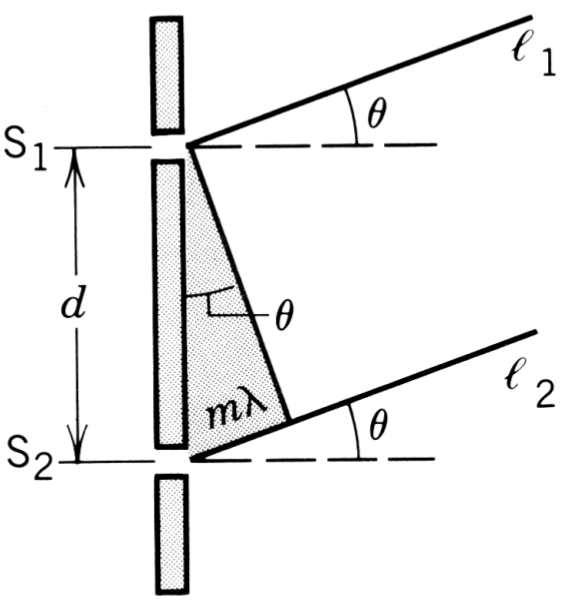
\includegraphics[width=0.3\textwidth]{./Exp9/pic/image1.png}
\caption{Geometry of the Double Slit}
\label{fig:slit}
\end{figure}

As you may convince yourself by looking at the graph, the difference in path between the two rays is
\begin{equation}
  \Delta l =d\sin\theta
\end{equation}

As in the lab about standing waves we can have different possibilities how these two rays add up. They can add up to form a node or they can add up to form an anti node (or something in between). To form a node every mountain shall be made lower and every valley shall be made higher. Therefore each hill from one wave should meet a valley from the other ray and vice versa. To get an antinode and therefore a maximum in the total motion of the wave every hill should meet a hill and every valley should meet a valley.
\begin{figure}[h]
\centering
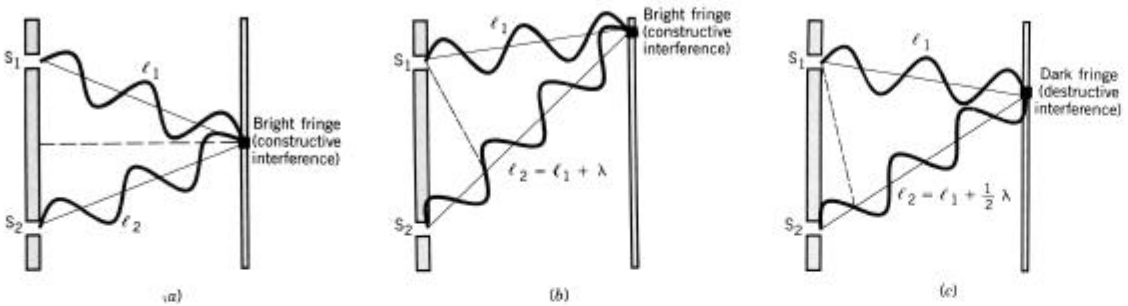
\includegraphics[width=0.8\textwidth]{./Exp9/pic/image2.png}
\caption{Young's Double Slit}
\end{figure}

How do we now achieve maximum intensity (node)? We always get this if the two waves are in phase which means that there fits an exact number of wavelength $m$ in the difference between the two waves, i.e.,
\begin{equation}
  \Delta l=m\lambda
\end{equation}
$m$ is also called the order. If we now put the two equations for $\Delta l$ together, we get
\begin{equation}
  d\sin\theta=m\lambda
  \label{eq:dsin}
\end{equation}
\begin{figure}[h]
\centering
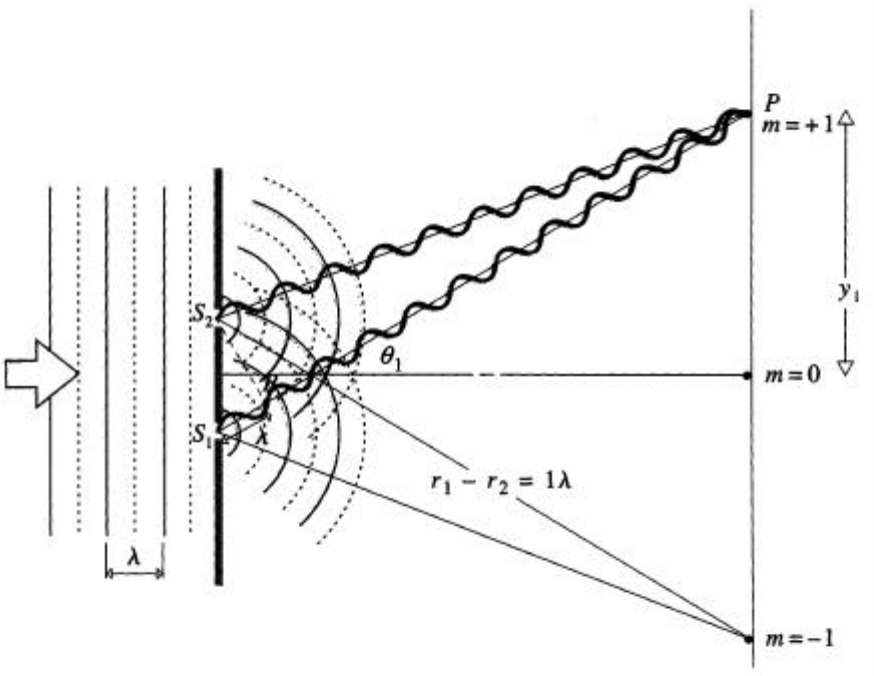
\includegraphics[width=0.6\textwidth]{./Exp9/pic/image3.png}
\caption{Interference of Light Coming from Two Small Slits}
\end{figure}

This tells us that given the order $m$ we can determine the wavelength of the light we see through the grating by reading off the angle. This also works the other way around; if we start with $m = 0$ at an angle of $0$ degrees and look for a particular color (wavelength), then each successive line of that color will be an additional order up (e.g. the third blue line you see as you increase your angle from 0 will be of order $m=3$ and  the third blue line you see as you decrease your angle from 0  will be of order $m=-3$).

\subsection{How to read a Vernier Scale}
With a usual ruler you can read distances up to a mm resolution. But if you would like to have a measuring device to read with a $0.1\, \mathrm{mm}$ resolution you have a problem. In principle you can scratch such a fine scale in the ruler, but in practice you can easily imagine that due to the width of the marks themselves such a scale would be almost impossible to read. That is why we use a trick and introduce a Vernier scale.\myskip

A Vernier scale works in the following way:

\begin{enumerate}[a)]
\begin{figure}[h]
\centering
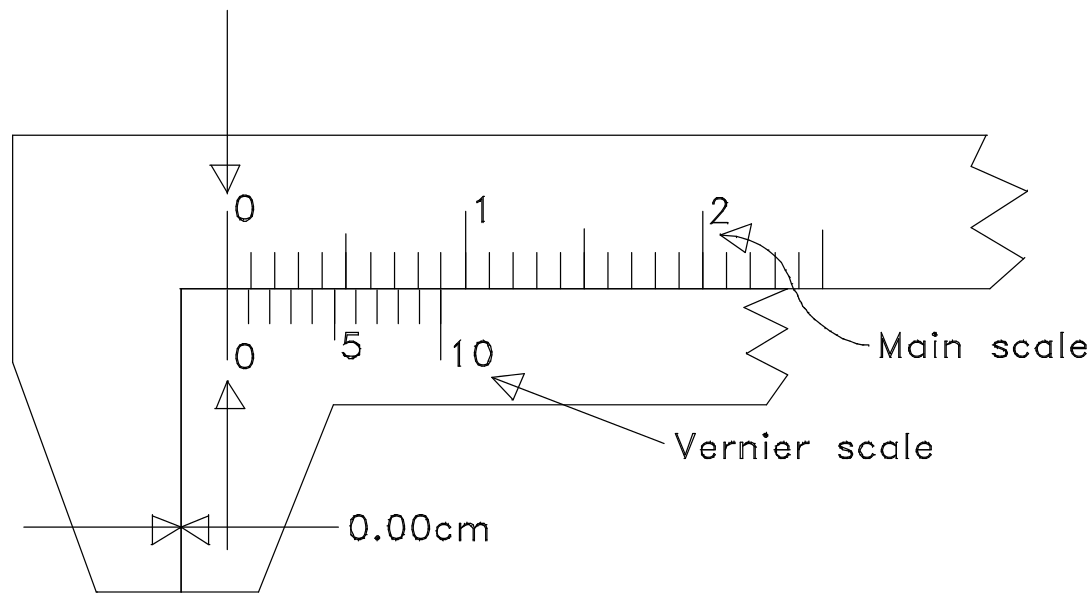
\includegraphics[width=0.5\textwidth]{./Exp9/pic/image4.png}
\end{figure}
\item If the zero points of the vernier and main scales are aligned, the first vernier division is 1/10 of a main scale division short of a mark on the main scale; the \engordnumber{2} vernier division is 2/10 of a main scale division short of the next mark on the main scale, etc. Note that the \engordnumber{10} vernier mark coincides exactly with a main scale mark.

\begin{figure}[h]
\centering
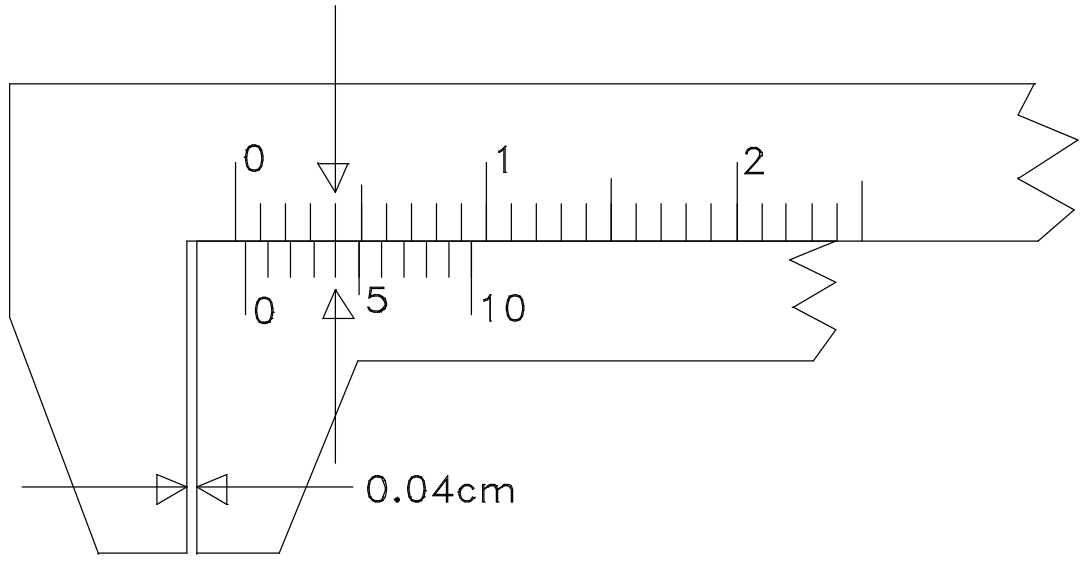
\includegraphics[width=0.5\textwidth]{./Exp9/pic/image5.png}
\end{figure}
\item If the vernier scale is now moved to the right until the \engordnumber{4} vernier division is lined up with the nearest main scale division to its right, the distance the 0 point of the vernier scale has moved past the 0 point on the main scale is 4/10 of a main scale division. Thus the vernier scale gives the fraction of a main scale division that the zero point of the vernier has moved beyond any main scale mark.
\begin{figure}[h]
\centering
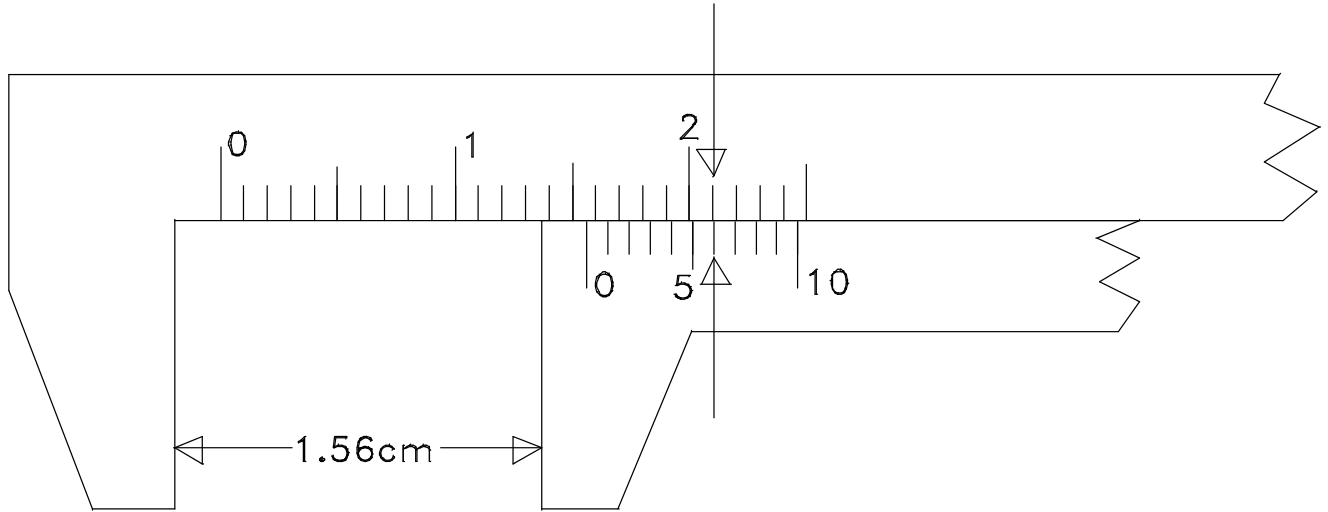
\includegraphics[width=0.5\textwidth]{./Exp9/pic/image6.png}
\end{figure}

\item In this last example, the zero line of the vernier scale lies between $1.5\,\mathrm{cm}$ and $1.6\,\mathrm{cm}$ on the main scale. The fraction of a division from $1.5\,\mathrm{cm}$ to the zero line can be determined as follows: Line number 6 of the vernier scale coincides with a line on the main scale, so the zero line on the vernier has moved 6/10 of a main scale division away from the main scale line 1.5. Hence, the reading, to the nearest hundredth, is 1.56. The maximum uncertainty is now $\pm 0.01\,\mathrm{cm}$, corresponding to the smallest division on the vernier scale. The use of the vernier has reduced the maximum uncertainty of the caliper measurement from $\pm 0.1\,\mathrm{cm}$ (without the vernier) to $\pm 0.01\,\mathrm{cm}$.
\end{enumerate}

In this experiment we will not use a simple Vernier scale since we do not measure distances, but we will use an angular Vernier scale to measure sub-divisions of angles. If you look at the main scale you will see that the scale is divided in half-degree steps. (You have slightly longer marks for the full degrees and shorter marks for the half degrees.) For angles the next smaller unit is not 1/10 th of a degree but minutes, which is 1/60 th of a degree. But since we can already read the scale up to 1/2 degree we need not have a Vernier scale with 60 divisions but with 30 divisions.\myskip

So you first use the 0 mark on the Vernier scale to read off the angle in degrees and if you are in between 0 and 30 minutes or 30 and 60 minutes. Then you look which of the markers on the Vernier scale exactly matches a mark on the other scale. So e.g. if the 0 mark on the Vernier scale is between 20.5 and 21 degrees and the \engordnumber{13} mark on the Vernier scale matches a mark on the degree scale we would have a reading of $20 + 1/2+ 13/60$ degrees or 20 degrees and 43 minutes.

\begin{figure}
\centering
\begin{subfigure}[b]{\textwidth}
  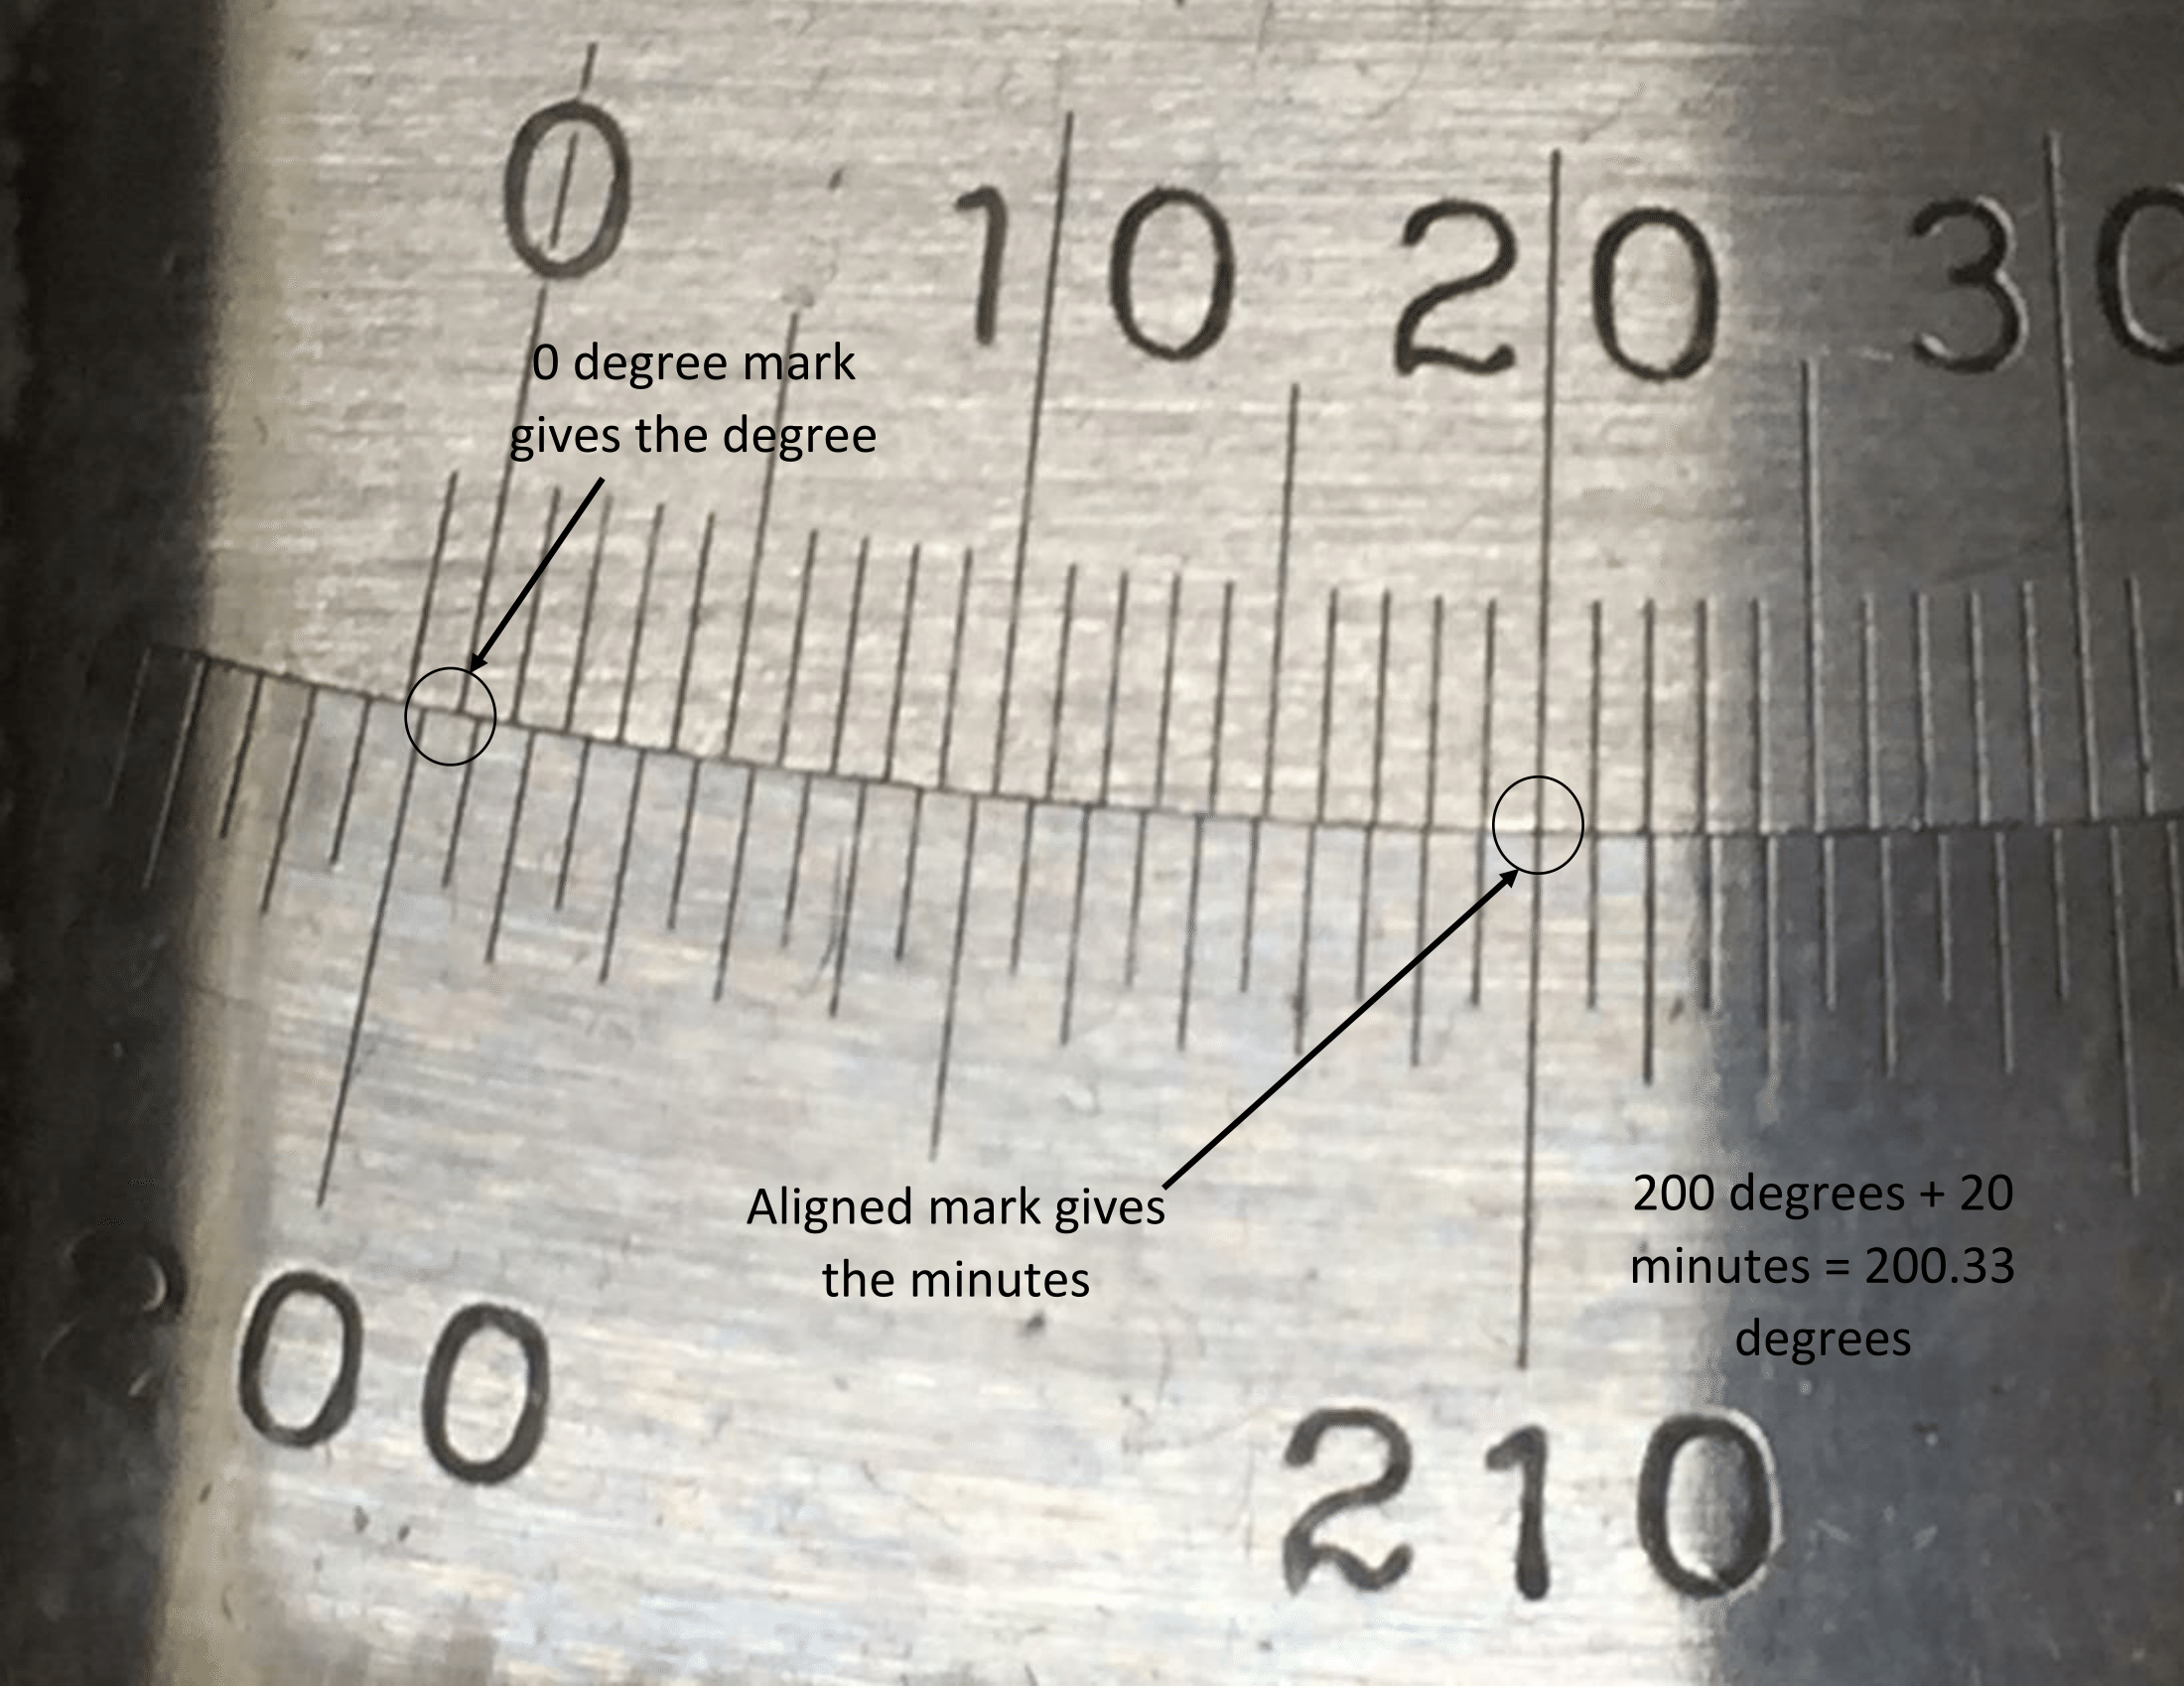
\includegraphics[width=0.85\textwidth]{./Exp9/pic/vernierexample1.png}
\end{subfigure}

\begin{subfigure}[b]{\textwidth}
  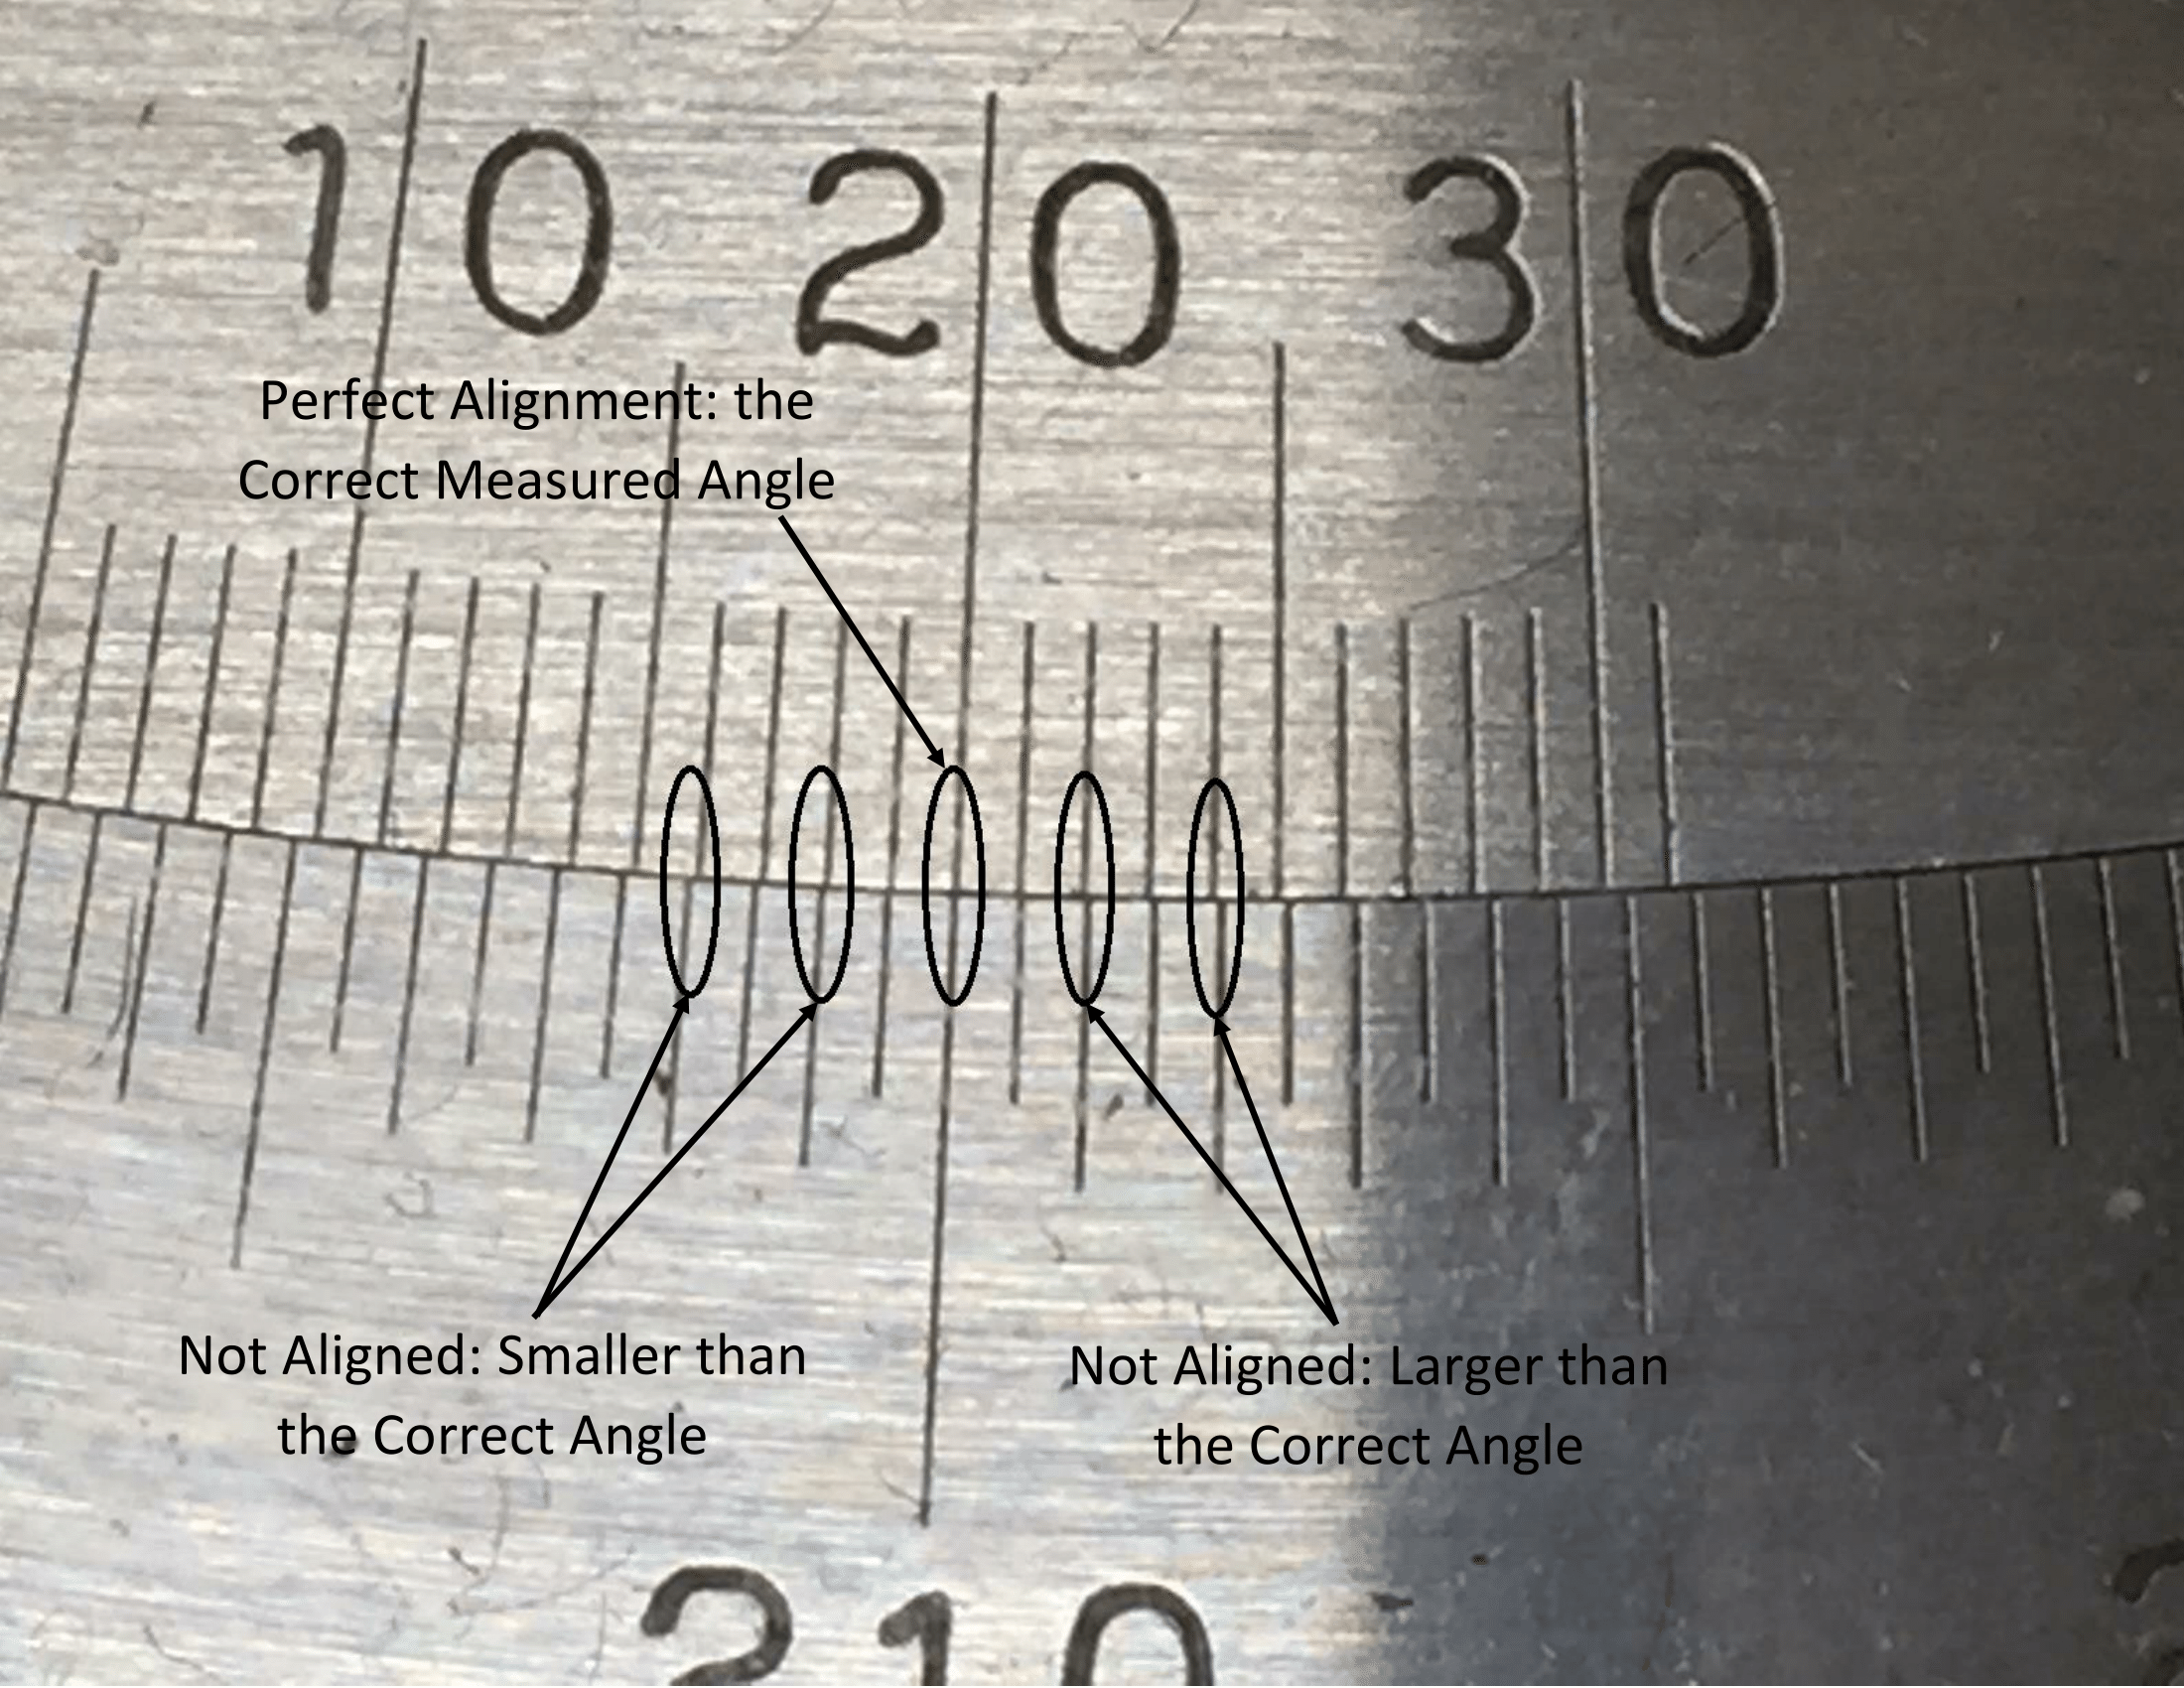
\includegraphics[width=0.85\textwidth]{./Exp9/pic/vernierexample2.png}
\end{subfigure}
\caption{A close-up of the angular Vernier scale used in the experiment including how to determine the minutes in detail.}
\end{figure}

\newpage

\section{Procedure}
\subsection{Adjusting the Spectrometer}
The first part of the experiment will basically include the procedure to set up the equipment. This should be done with as much care as possible. Only then we will be able to measure the wavelength on the limit of our apparatus. If you don't set up the spectrometer correctly you will get systematical errors, which will negatively impact your data.

\begin{figure}[h!]
\centering
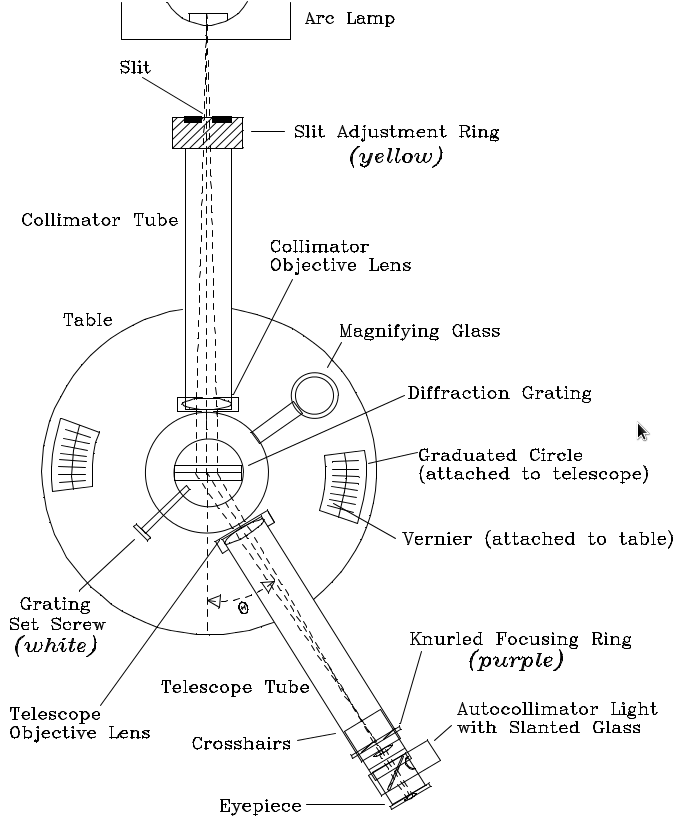
\includegraphics[width=0.75\textwidth]{./Exp9/pic/image7.png}
\caption{Schematic of the Spectrometer}
\end{figure}

\begin{figure}
\centering
\begin{subfigure}[b]{\textwidth}
  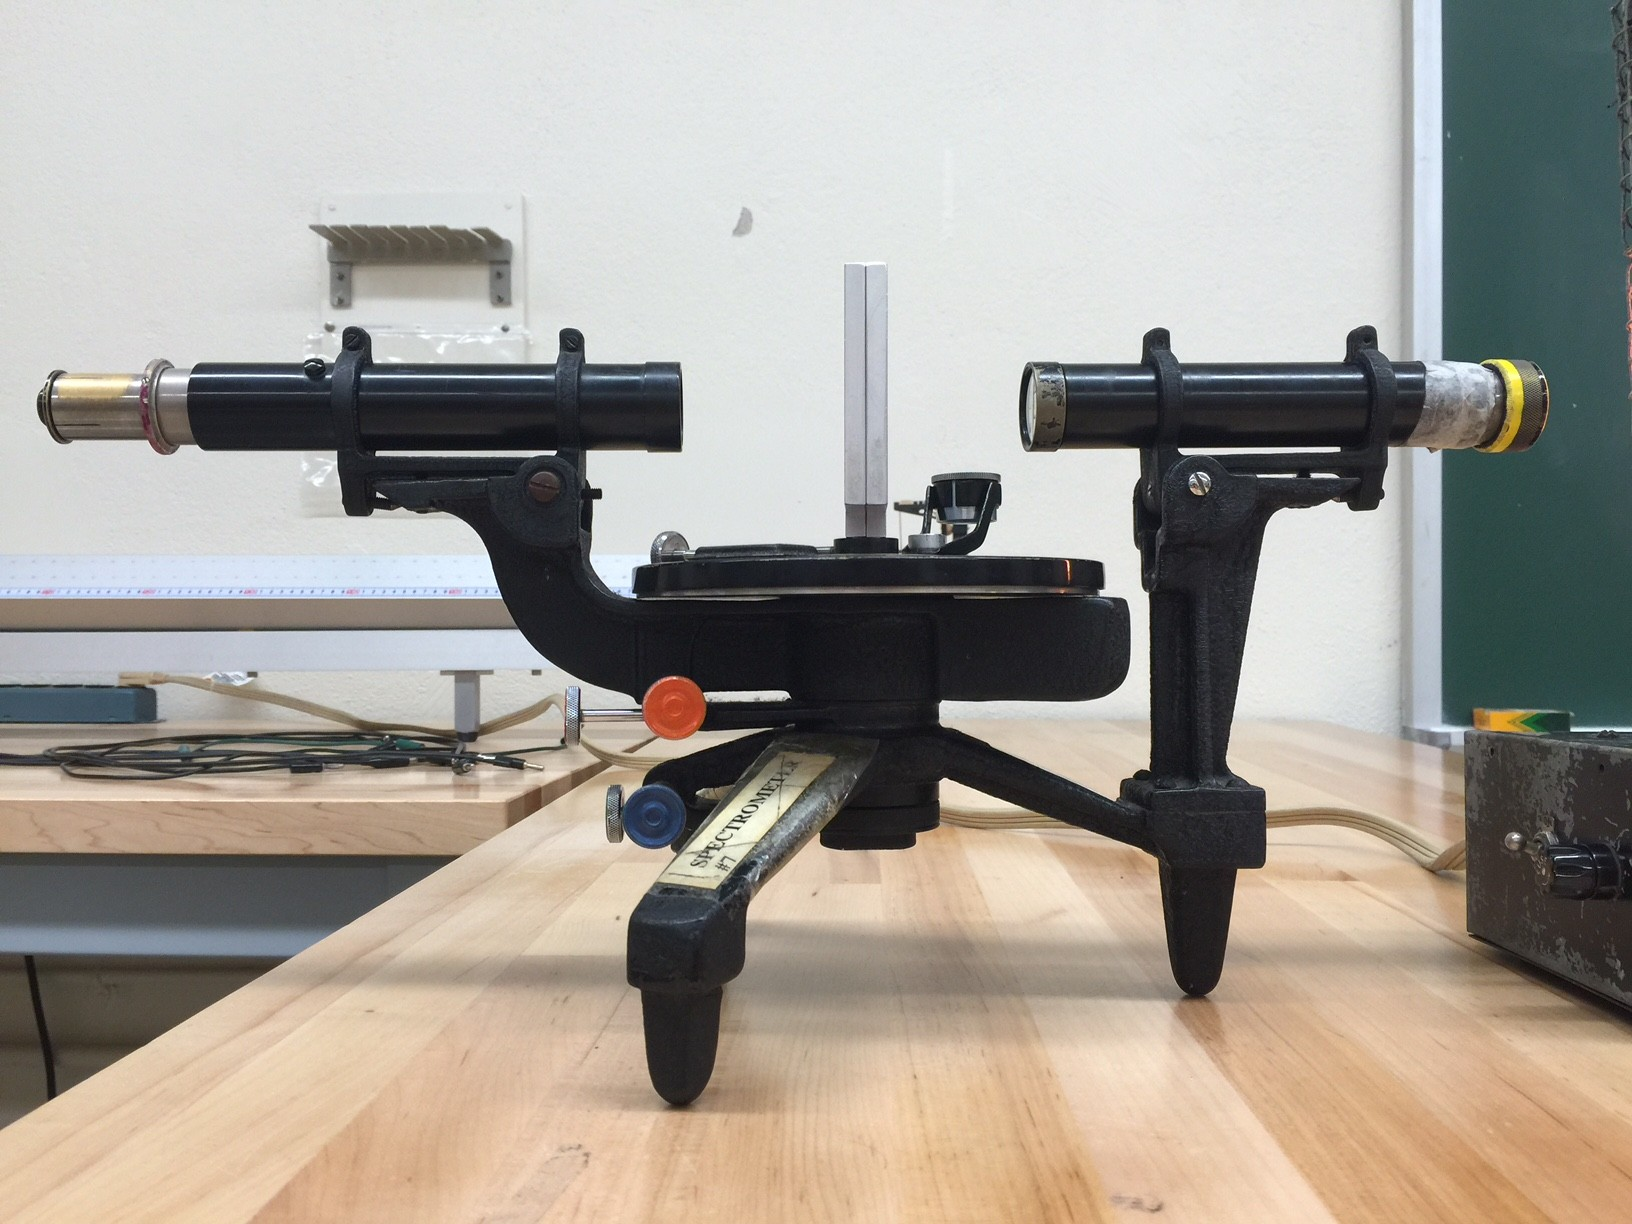
\includegraphics[width=0.75\textwidth]{./Exp9/pic/spectroside.jpg}
  \subcaption{A side view of the spectrometer.}
\end{subfigure}

\begin{subfigure}[b]{\textwidth}
  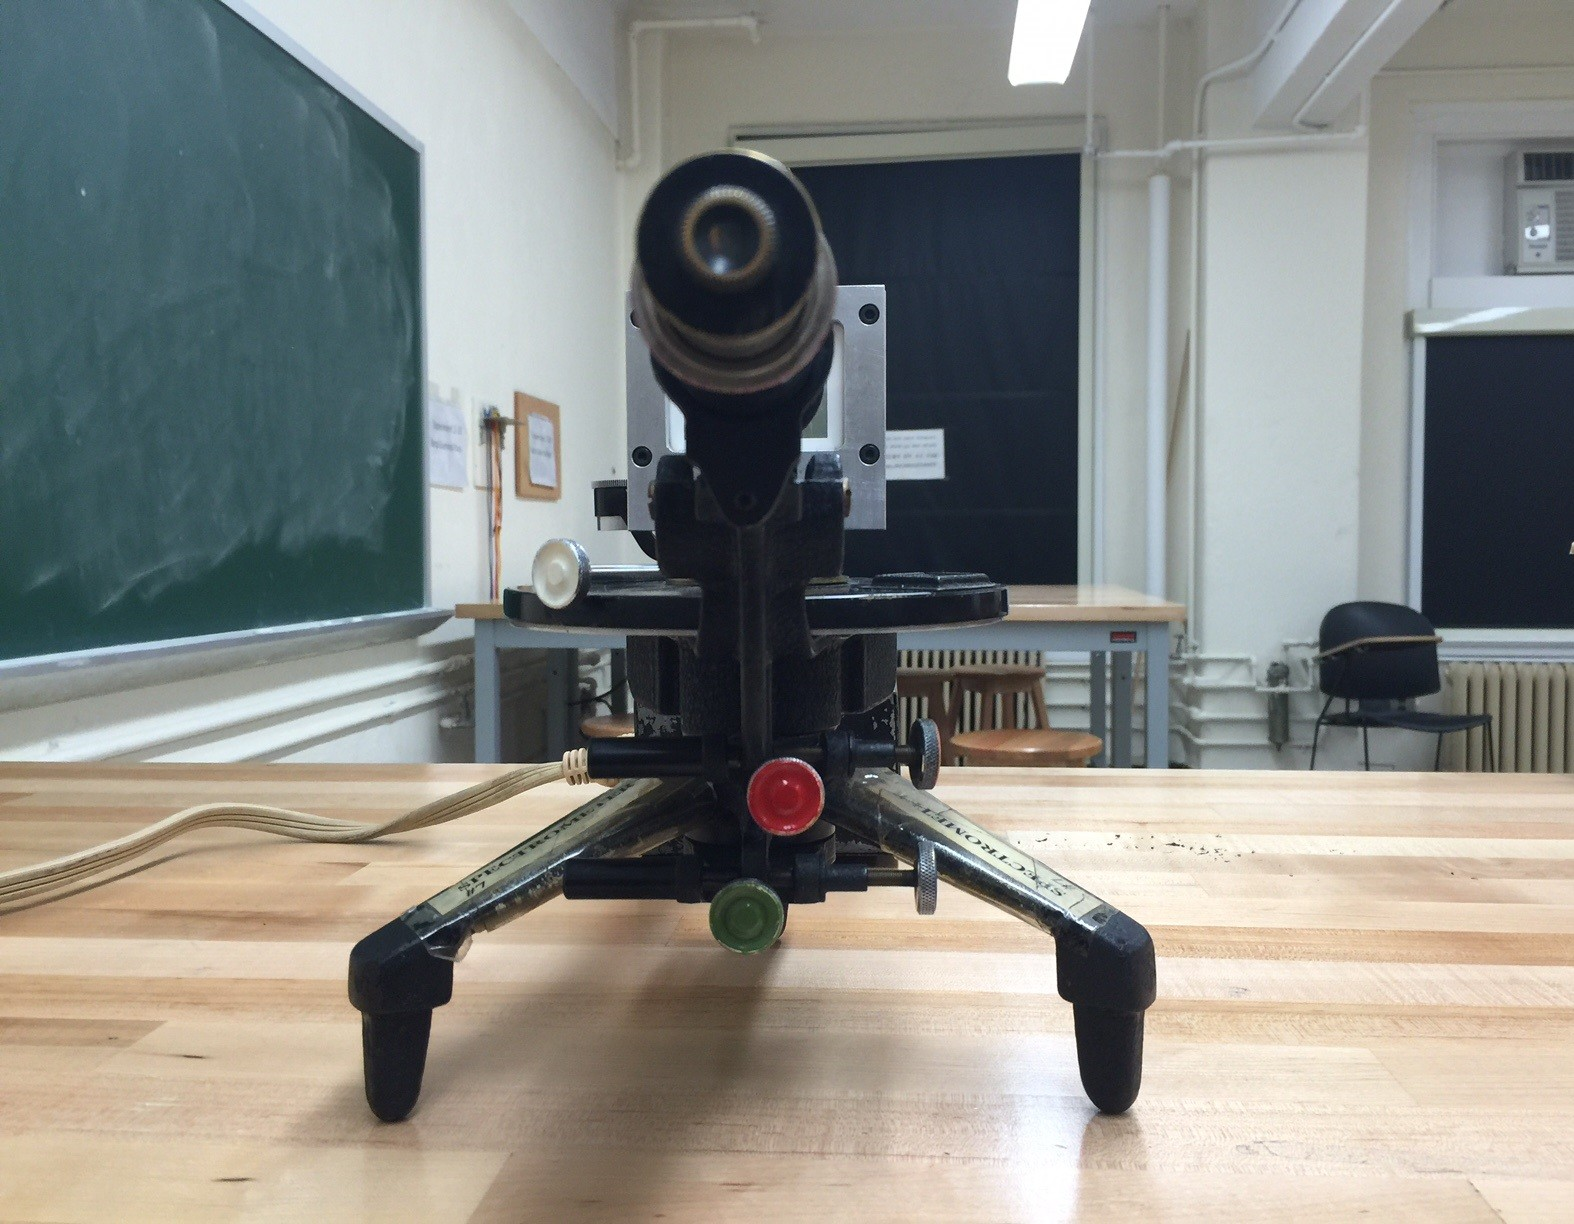
\includegraphics[width=0.75\textwidth]{./Exp9/pic/spectrofront.jpg}
  \subcaption{A front view of the spectrometer.}
\end{subfigure}
\end{figure}

\subsection{Obtaining the Lattice Constant}
 After adjusting the spectrometer we will measure the yellow line of a Helium discharge lamp. Since we know that the wavelength of this light is $\lambda = 5.8756\times 10^{-7}\,\mathrm{m}$, we can determine the lattice constant of the grating quite accurately. Even though the lattice has written on it 600 lines/mm (which is only an approximate value anyway), we want to get the lattice constant with 5 relevant digits and not just 3, and this means that we have to measure it!

\subsection{Measuring the Spectrum of Hydrogen Atoms}
With the lattice constant determined in the previous part we now measure the wavelength of the light emitted from the Hydrogen discharge lamp.

\section{Step by Step List}
\subsection{Adjusting the Spectrometer}
\begin{enumerate}
\item Remove the grating from the holder and close the green knob.

\item Rotate the yellow knob such that the slit is about half open.

\item Look trough the eyepiece and turn the purple focusing ring until you see a sharp image of the slit.

\item Loosen the red knob and move the telescope tube until the cross hair is in the middle of the slit. Tighten red knob.

\item Now open the green knob and turn the tabletop such that the 0 mark from the Vernier scale with the magnifying glass is lined with either the 180 or the 360 from the outer scale. (Always use only this Vernier scale and don't switch to the other one in between)

\item Close the green knob (and don't open it again for the rest of the experiment!).

\item Now you can fine adjust the relative position of the inner and outer scale by turning the blue knob. Make sure that the lineup between the 0 on the Vernier and the 180/360 is done as careful as possible. (For some of the spectrometers there is a small mark to the left of the 0 mark on the Vernier scale. Make sure that you line up the 0 mark and not this extra mark with the 180/360.)

\item Now put the grating in the holder such that it is perpendicular to the telescope tube-collimator tube line. Close the white screw to lock the grating.
\end{enumerate}

\subsection{Obtaining the Lattice Constant}
\begin{enumerate}
\item Switch on the Helium lamp and line the spectrometer up such that you can see the slit well illuminated by the lamp as you look through the spectrometer.

\item Put the black cardboard over the front end of your collimator tube and you can use the black piece of cloth over the spectrometer to block light from the surrounding. The spectrum lines can be quite dim and any outside light will make it very hard to find the right ones. Make sure the room lights are switched off for these measurements. Lower-intensity desk lamps are provided to read the scale on the spectrometer.

\item Open the red knob and move the telescope tube to the left until the crosshair is in the center of the yellow line. You should first see a few blue and green lines, then the isolated yellow line and then red lines (the yellow line should be somewhere around 20 degrees).

\item Note down the angle in degrees and minutes at which you see the \engordnumber{1} order of the yellow line. Do the same on the right side and average these two numbers.

\item Use the average and plug it into the grating equation ($m=1$) to determine the lattice constant $d$ (at least 5 relevant figures).

\item How many lines per mm does this lattice constant correspond to?

\item Can you also see the \engordnumber{2} order and \engordnumber{3} order yellow lines on either side?
\end{enumerate}

\subsection{Measuring the Spectrum of Hydrogen Atoms}
\begin{enumerate}
\item Now switch off the helium lamp and set up the spectrometer for the hydrogen lamp.

\item The light purple line you see in the middle is the $0^{\mathrm{th}}$ order and not yet one of the lines we are going to measure.

\item There are 4 visible lines for each order the Hydrogen spectrum. One red (furthest out), one greenish blue, one purple blue and one dark purple. The dark purple line is very faint and you may not be able to see it, so please don't despair and just focus on the three visible lines.

\item Measure the angles of the 4 lines on both sides and average the angles.

\item What are the wavelengths, $\lambda$ for each of the 4 colors of light?

\item How many orders do you see on either side? (for example, look for the red line and count how often it appears as you go further out from $0$ degrees)

\item Do the higher orders overlap? (i.e. do you ever see the first color of one order before seeing the last color of the previous order?)
\end{enumerate}

\subsection{Analyzing the Data}
\begin{enumerate}
\item Put together formulas ({\ref{eq:lambda}}) and ({\ref{eq:dsin}}) to derive an equation for for $n_i$.
\item Use your data and the value for $R$ from above and $n_f=2$ to determine $n_i$ for each color (it should not matter which order you choose). Don't worry about calculating the uncertainty because it is an absolute nightmare  with that equation.
\item $n_i$ should be an integer number labeling from which initial atomic shell the electrons in the hydrogen atoms fell to the \engordnumber{2} atomic shell. Are your results integers (or close to one)?
\item Which color corresponds with the smallest electron jump (i.e. for which color was $n_i$ the lowest)? Explain why you could have predicted that anyway!
\item Within how many \% have you been able to measure the data? Compare that to other experiments you have performed in this course!
\item Discuss briefly the factors that determine the uncertainty in your measurements. Which of them are random, which systematic?
\end{enumerate}

\newpage
\section{Lab Preparation Examples}
\underline{Hydrogen Spectrum:}
\begin{enumerate}
\item What is the wavelength of emitted if an electron in a hydrogen atom makes a transition from $n_i=3$ to $n_f=1$?

\item For a hydrogen atom give all the transitions that fall within the visible range of the light spectrum (i.e. between $\lambda_{\mathrm{min}}=400\,\mathrm{nm}$ and $\lambda_{\mathrm{max}}=800\,\mathrm{nm}$). Give the transitions in the following form:
A transition from energy level $n_i=3$ to $n_f=1:3 \rightarrow 1$.\myskip

Hint: It may be simplest to calculate the energies $\lambda_{\mathrm{min}}=400\,\mathrm{nm}$ and $\lambda_{\mathrm{max}}=800\,\mathrm{nm}$ correspond to. Then make a list of $E_{n}$ and choose the differences between the energy level that fit in the calculated range.

\item What wavelengths do the transitions in the previous problem correspond to?
\item If you look at the light of an object at high temperature (e.g., a normal light bulb), you will find that it usually emits a continuous spectrum without any gaps or lines in it. (This is due to the effect that the atoms in a solid (or plasma) are so close together that they disturb each other so strongly that the initially sharp transition lines of the atoms get so broadened that they appear as a continuous spectrum.)\myskip

But if you now look at the spectrum of the sun (or another star), you will find a continuous spectrum that has a number of sharp black lines, so no (or almost no) light of that frequency reaches you; the light of that frequency is missing in the spectrum. These black lines are at exactly the same positions where you would see the colored lines in emission spectra (that is what we do in lab) of the elements present on the sun. For example since hydrogen is present on the sun we will find black lines at the
wavelength calculated in 3.\myskip

Can you give a short explanation of how we get these inverse spectra (compared to the ones we see in the lab from emission spectra) from the sun?
\end{enumerate}

\noindent\underline{Spectrum with a Grating:}
\begin{enumerate}\setcounter{enumi}{4}
\item What is the lattice constant $d$ if the lattice has 400 lines per mm?
\item If you have a grating with 600 lines per mm at what angle would you observe the $m=1$ maximum for a wavelength of $600\,\mathrm{nm}$?
\item If you have $d = 10^{-1}\, \mathrm{m}$ and $\lambda = 1\,\mathrm{cm}$. at what angles will you see the maxima for $m=1, 2, 3$?
\end{enumerate}
